\documentclass[12pt]{article}
\usepackage[margin=1in,letterpaper]{geometry}
\usepackage{amsmath}
\usepackage{amsfonts}
\usepackage{graphicx}
\usepackage{hyperref}
\hypersetup{
    colorlinks = true,
    citecolor={black},
    linkcolor={red}
}
\usepackage{titling}
\posttitle{\par\end{center}}
\setlength{\droptitle}{0pt}
\begin{document}
\title{Crowd Segmentation Progress}
\author{\today}
\date{}
\vspace{-50pt}
\maketitle
\vspace{-70pt}
\section{Problem Formulation}
 The goal of quality evaluation is two-folds. Given N worker responses, find: 
 \begin{enumerate}
\item the quality of the bounding boxes (BB) drawn by worker 
\item the best proposed region for a given object in an image
 \end{enumerate}
\section{Key Assumptions and Intuitions}
\begin{enumerate}
\item In literature, there are scoring functions that require ``ground truth" and ones that are ``unsupervised". 
\item If a worker's response differs greatly from the ground truth, then work quality ($Q_w$) is low. 
\item If most of the workers' response differ greatly from ground truth for a particular image, then task difficulty ($D_t$) should be high. As a corollary, if the spread of the $J_i$ distribution is large, then $D_t$ should also be high.
\end{enumerate}
To compute the latent quantities $Q_w$,$D_t$, we propose an iterative EM-like algorithm, where at every step, we assume that the ground truth bounding box ($BB_G$) is the current estimate of the maximum likelihood region. The maximum likelihood region is constructed by adding in sub-regions from a tile-graph. 
\section{Generative Process}
\begin{figure}[ht]
\centering
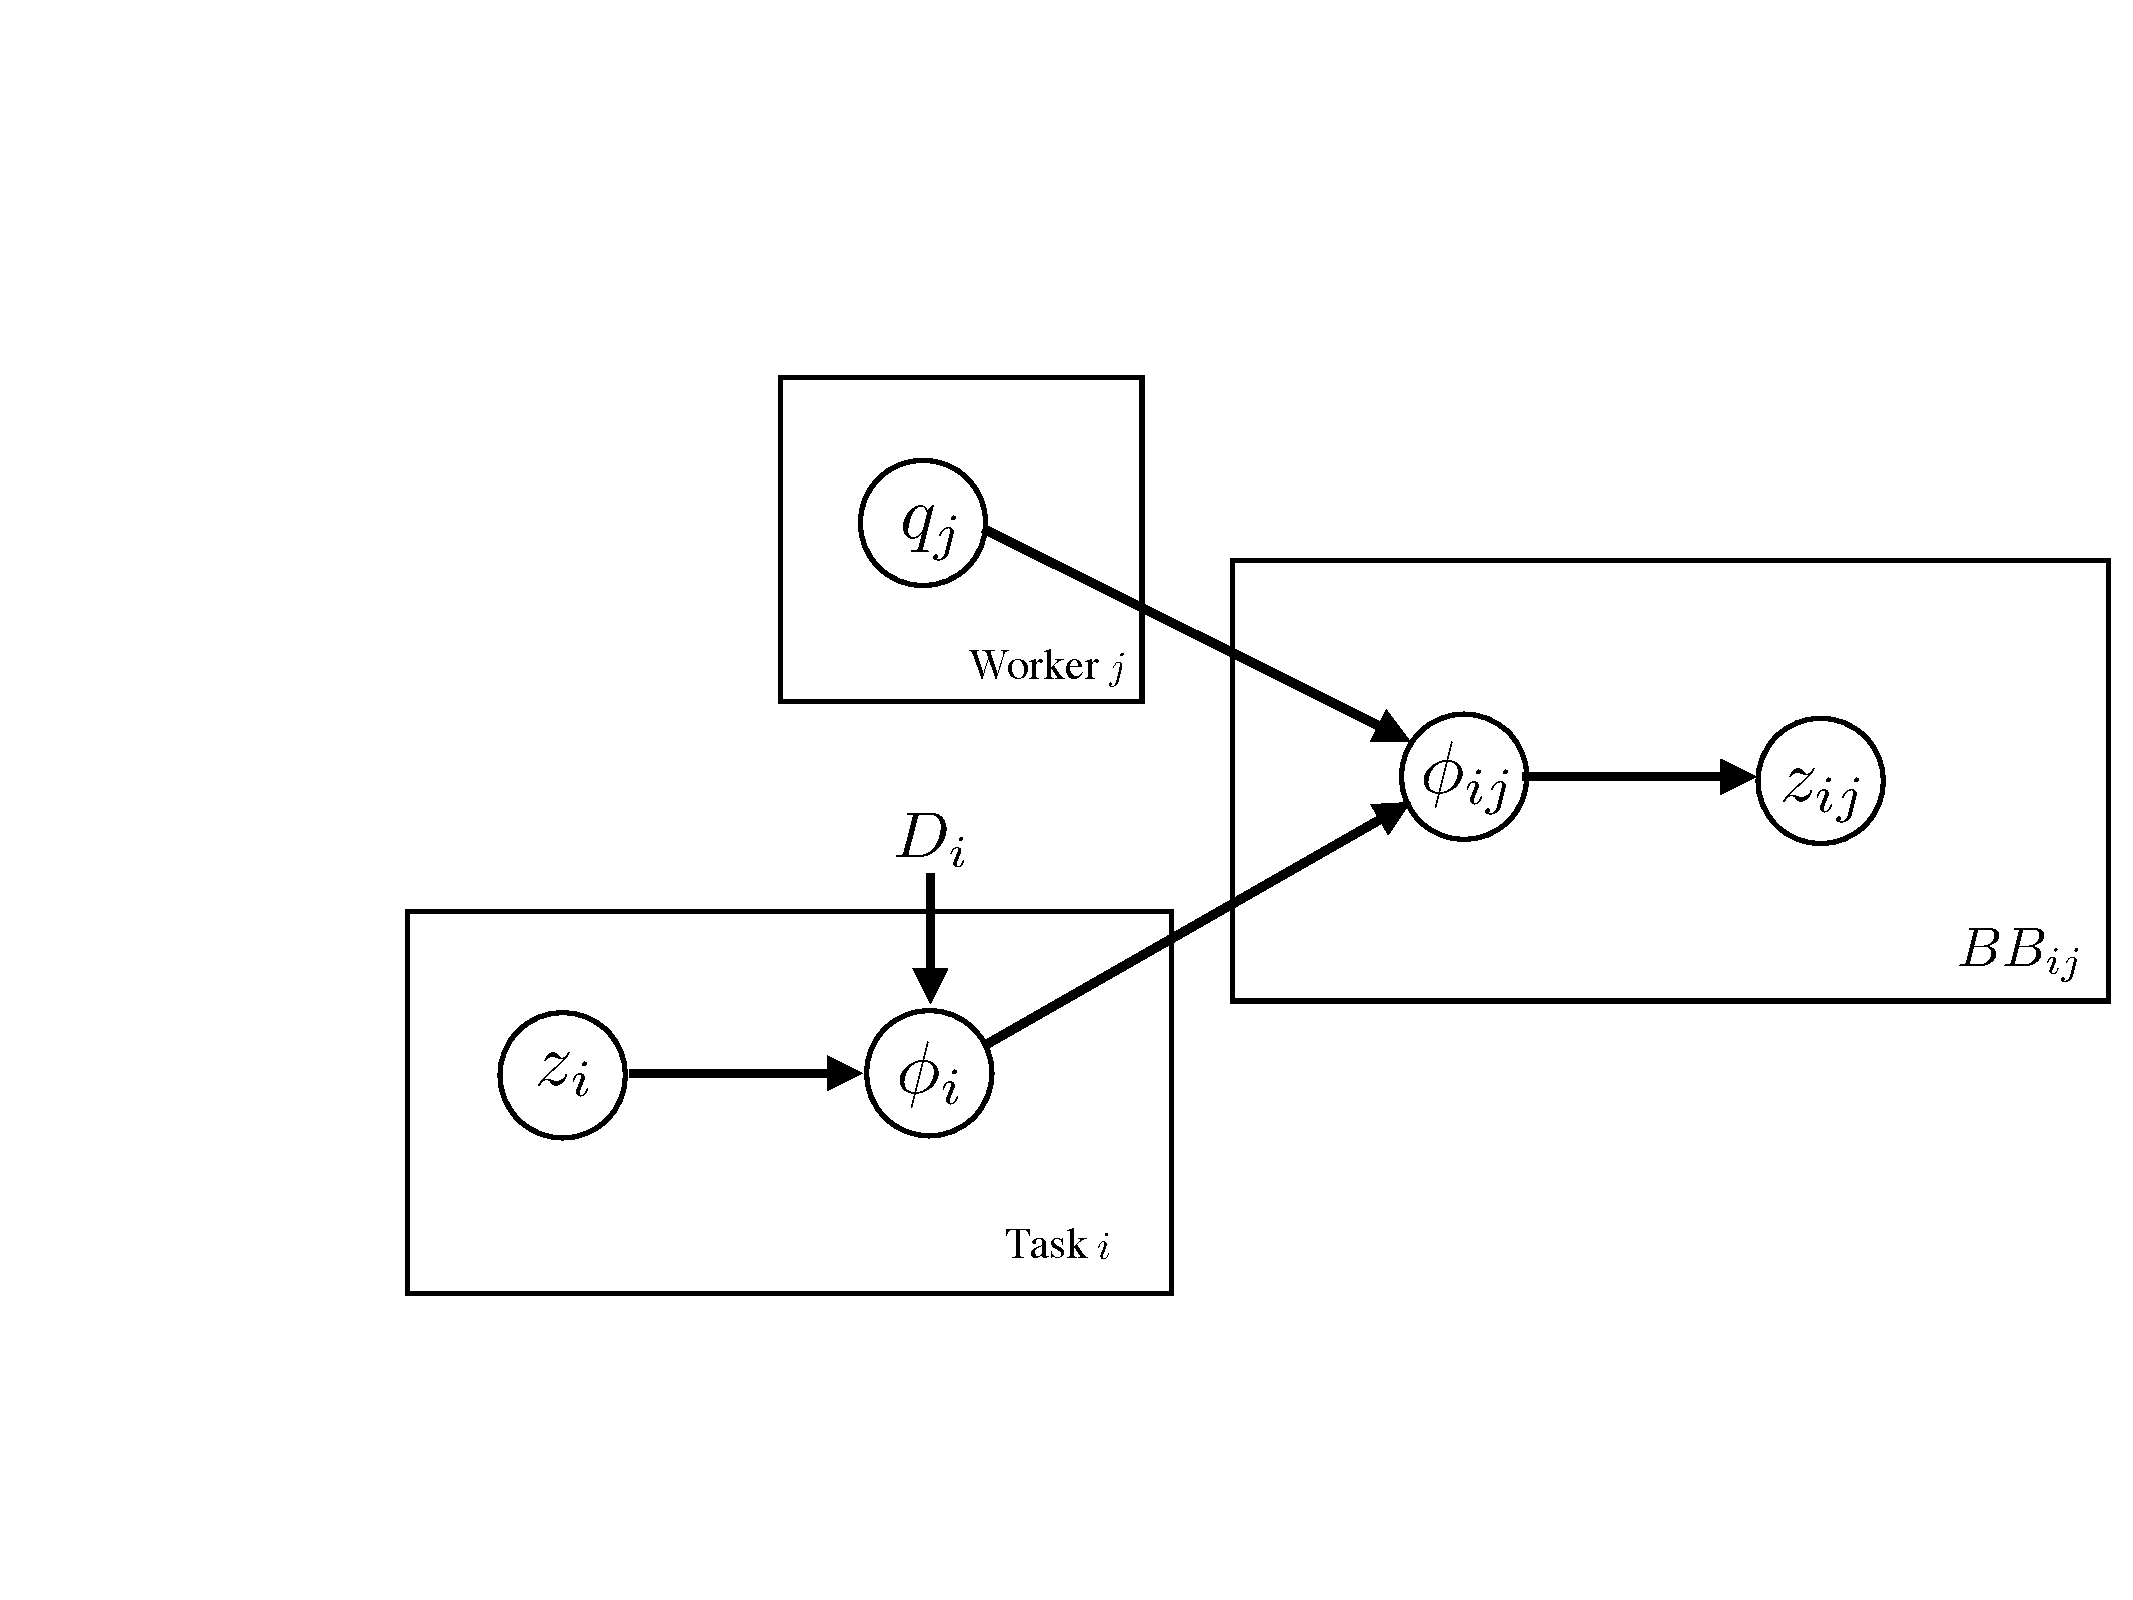
\includegraphics[trim=1cm 5cm 1cm 5cm,width=0.8\linewidth]{plots/generative_pgm.pdf}
\caption{Proposed probabilistic graphical model for crowdsourcing image segmentation.}
\end{figure}
The generative model is inspired by \cite{Welinder2010}, the process is as follows:
\begin{itemize}
\item A task is defined by an object-image pair i : 
\begin{itemize}
\item $z_i$ is hidden variable that completely describes the ground truth BB from the image (e.g. set of all points in $BB_G$).
\item  $\phi_j$ is some descriptive image-related quantity extracted from $BB_G$ This can either be a 1-D scalar aggregate or a multidimensional quantity. (e.g. boundary complexity of the image boundary)
\item $J_i$ is the set of all workers j that annotated the object-image. 
\item $D_i$ is the task difficulty of object-image i.  The $\phi_j$ image summary is determined by both the objective description of $BB_G$ ($z_i$) and the difficulty of the task. The task difficulty is a measure of how far off are most of the worker's responses compared to $BB_G$.  
\begin{equation}
D_i = \sum_{j\in J_i} dist(\phi_j,\phi_i)
\end{equation}
Here, we can model the distribution of $\phi_i$ as :
$$p(\phi_i|z_i) = N(\phi_i;z_i,D_i^2)$$
This agrees with our intuition that in a distribution of image descriptions for all workers, the larger the spread means that the task is difficult. The distribution is centered around $z_i$ (i.e. complete description of $BB_G$).
\end{itemize}
\item By definition, we assume here that task difficulty is completely a result of the image itself and independent of any worker qualities. The worker j is described by the quality of work that he produces parameterized as $q_i$. We can also try to model user expertise, but this is less important in salient, common-object segmentation. If we chose to take the prior appraoch, we assume that $q_i$ only parameterizes the vision-related quantities affecting worker j's judgement on $\phi_{ij}$.
\begin{equation}
q_j = dist(\phi_{ij},\phi_i)
\end{equation}
\item Both the characteristics of the ground truth BB ($\phi_i$) and the worker's ability to segment the image ($q_i$) would determine how the worker would percieve the image($\phi_{ij}$) and what worker's BB would look like ($z_{ij}$).
%\item Finally, the characteristics of the BB drawn by worker i is just a summary of the BB drawn by worker i ($BB_i$)
\end{itemize}
\section{Proposed Functions for $\Phi$}
\paragraph{Boundary-based:} Boundary complexity. Set of fixed-number of interpolated boundary points for computing distance.\cite{Vittayakorn2011}
\paragraph{Contrast-based:} how close is BB to regions of contrasts detected by CV algorithms (saliency maps, Bayesian Matting) or edge detectors 
\paragraph{Area-based:} Precision, Recall
\section{Preliminary Experiment}
We ran a preliminary experiment where each HIT consisted of one annotation task for a specific pre-labelled object in the image, as shown in Fig.\ref{interface}. There is a total of 46 objects in 9 images from the MSCOCO dataset\cite{Lin2014}. These objects and images are intentionally chosen so that they represent a variety of image difficulty (based on object clutter-ness) and potential logical error and level of ambiguity. The average number of objects annotations that each worker completed was 10.16. The average time to complete each HIT is 83.96 seconds and workers are compensated for 5 cents per HIT.  For each object, we collected annotations from a total of 40 independent workers.
\par There are two sets of annotations that we used as ground truth comparison for computing these metrics: gold-standard annotations cross-matched with MSCOCO (\texttt{[COCO]}) and detailed annotation boundaries drawn by me with the same web interface (\texttt{[Self]}). Note that some of the COCO annotations lack exact cross matches. The metrics computed for objects that are not in the COCO database are flagged and not used for computing the evaluation metrics. However, inexact annotations of the same object (e.g. book-labelled object with only book cover annotation) is still incorporated in the computed metrics.

\begin{figure}[ht]
\centering
\fbox{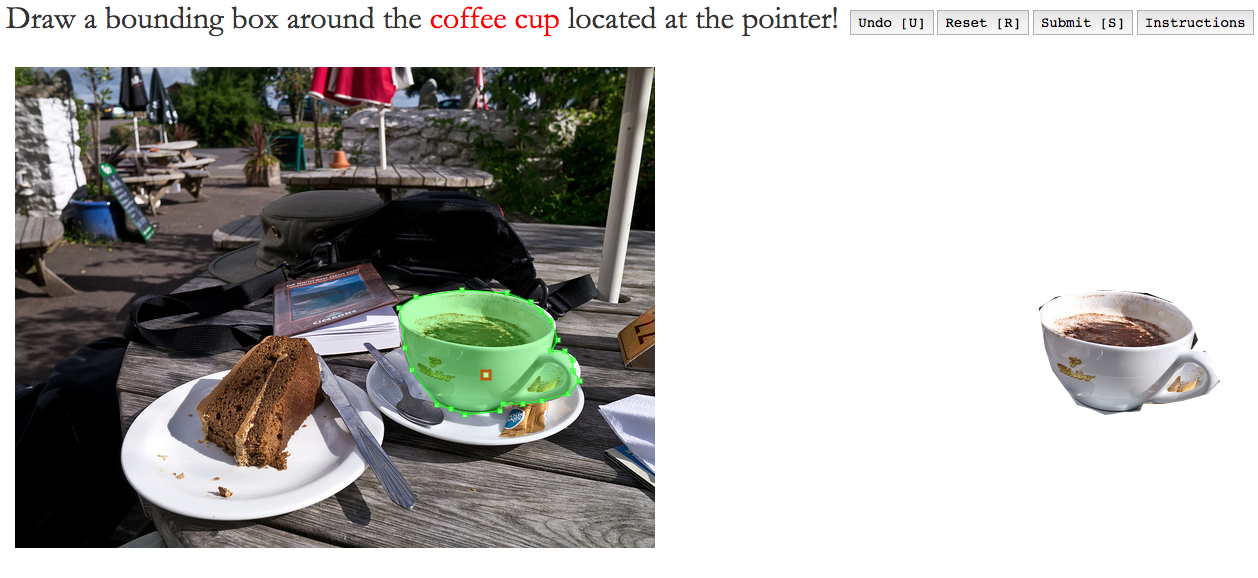
\includegraphics[width=0.9\linewidth]{plots/interface.png}}
\caption{An example can be seen  \href{http://crowd-segment.herokuapp.com/segment/COCO_train2014_000000000127/10/}{here}.}
\label{interface}
\end{figure}
\subsection{Data Observations}
\begin{itemize}
\item Most workers makes decent annotation that closely follows the ground-truth BB, below a threshold is mistakes are likely due to task ambiguity.
\item Both the number of task per worker and average time in a task follows a Pareto-like distribution, which is typical for crowdsourcing applications.
\item We are interested in whether our data agrees with Assumption \#2 and \#3 regarding work quality and task difficulty. 
%If a worker's response differs greatly from the ground truth, then work quality ($Q_w$) is low. 
%If many of the worker's response differs greatly from ground truth for a particular image, then task difficulty ($D_t$) is high.

\end{itemize}

\begin{table}[h]
\centering
\begin{tabular}{lrr}
\hline
 All              &   Mean &    SD \\
\hline
 Precision [COCO] &  0.869 & 0.227 \\
 Recall [COCO]    &  0.897 & 0.132 \\
 Jaccard [COCO]   &  0.789 & 0.227 \\
 Precision [Self] &  0.864 & 0.206 \\
 Recall [Self]    &  0.901 & 0.145 \\
 Jaccard [Self]   &  0.785 & 0.219 \\
\hline
\end{tabular}
\begin{tabular}{lrr}
\hline
Filtered                &   Mean &    SD \\
\hline
 Precision [COCO] &  0.931 & 0.068 \\
 Recall [COCO]    &  0.917 & 0.07  \\
 Jaccard [COCO]   &  0.858 & 0.082 \\
 Precision [Self] &  0.918 & 0.076 \\
 Recall [Self]    &  0.925 & 0.073 \\
 Jaccard [Self]   &  0.858 & 0.086 \\
\hline
\end{tabular}
\caption{Left: Statistics for all workers; Right: for good workers only [metric$\geq$0.6]}
\label{basic_stat}
\end{table}
\subsection{Fitting Procedure}
We are interested in figuring out what functional form these $\Phi$ functions are distributed as. We fitted the histograms against 84 different probability distribution functions\footnote{Most of the functions in  \href{https://docs.scipy.org/doc/scipy/reference/stats.html}{scipy.stats}:\tiny{[alpha, anglit, arcsine, beta, betaprime, bradford, burr, cauchy, chi, chi2, cosine, dgamma, dweibull, expon, exponpow, exponweib, f, fatiguelife, fisk, foldcauchy, foldnorm, frechet\_l, frechet\_r, gamma, gausshyper, genexpon, genextreme, gengamma, genhalflogistic, genlogistic, genpareto, gilbrat, gompertz, gumbel\_l, gumbel\_r, halfcauchy, halflogistic, halfnorm, hypsecant, invgamma, invgauss, invweibull, johnsonsb, johnsonsu, ksone, kstwobign, laplace, levy, levy\_l, loggamma, logistic, loglaplace, lognorm, lomax, maxwell, mielke, nakagami, ncf, nct, ncx2, norm, pareto, pearson3, powerlaw, powerlognorm, powernorm, rayleigh, rdist, recipinvgauss, reciprocal, rice, semicircular, t, triang, truncexpon, truncnorm, tukeylambda, uniform, vonmises, vonmises\_line, wald, weibull\_max, weibull\_min, wrapcauchy]}}, using the maximum-likelihood estimators of these distributions. Then, a  Kolmogorov-Smirnov test  assessed the statistical significance of whether the fitted function and the data follow the same distribution. We quantify the best fits using minimal residual sum-of-square (RSS) and the p-value resulting from the KS-test.  To preserve the tails of these distributions, no filtering for selecting good workers only was done in the fitting procedure. We also explicitly enforce a fixed range so that each $\Delta x$  is the same. 

\subsection{Overall Distribution}
\begin{figure}[ht]
\centering
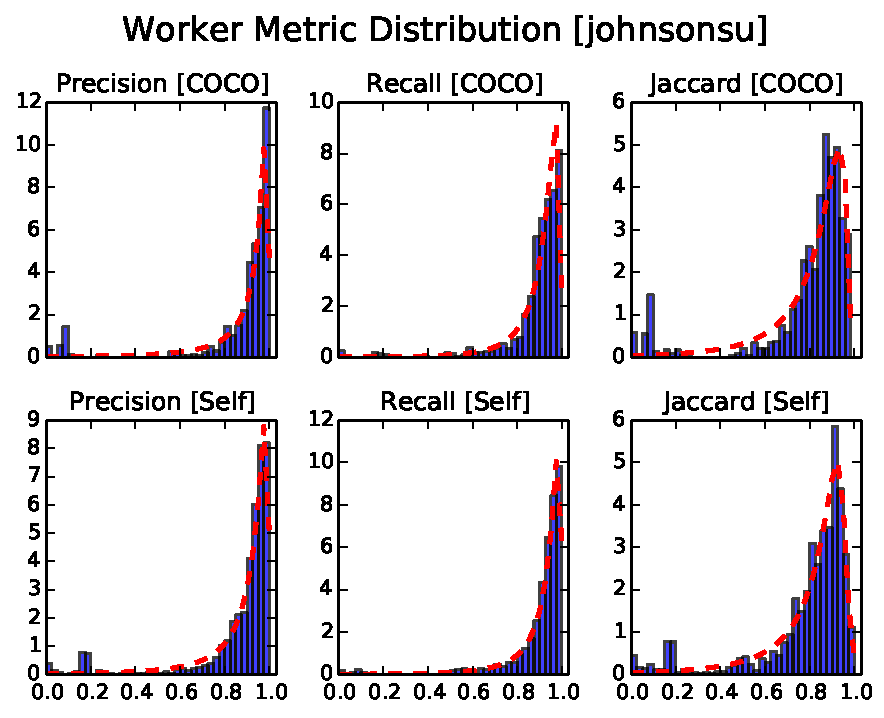
\includegraphics[width=0.45\linewidth]{plots/johnsonsu_fitted_metric_histogram.pdf}
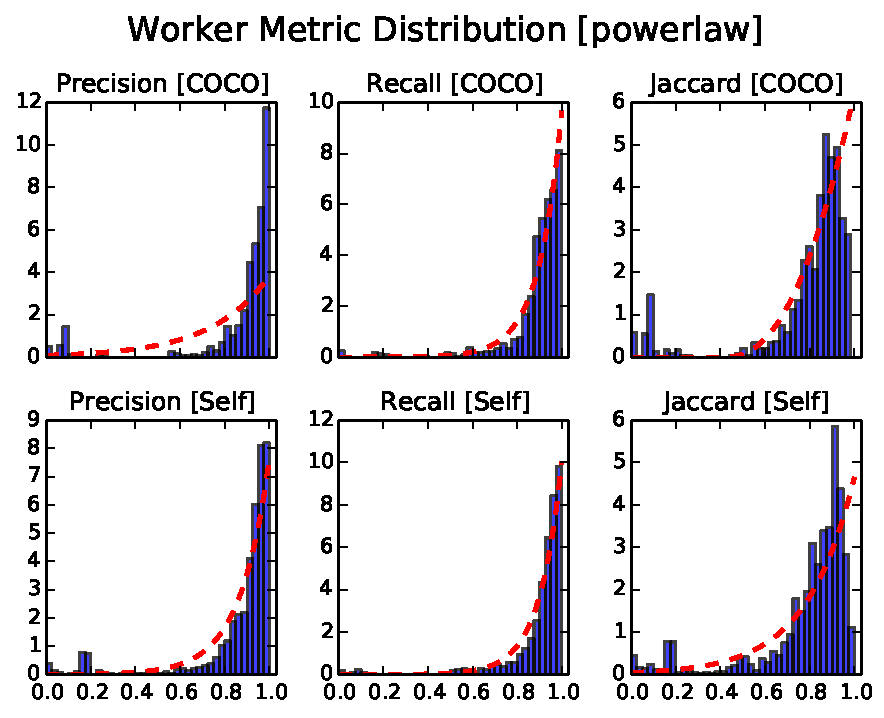
\includegraphics[width=0.45\linewidth]{plots/powerlaw_fitted_metric_histogram.pdf}
\caption{Normalized histogram of metric values, fitted with a Johnson SU (Left) and Power law distribution(Right). }
\label{metric_hist}
\end{figure}


\par For the overall distribution, we plot the metrics computed from all tasks submitted by all workers. The histogram distribution (fixed bin size =30) of these metrics resembles a long-tail, exponential-decaying distribution. There are many pdfs that fits one metric but not another. The distribution that yields the best fits for all metrics is the Johnson SU distribution, as summarized in Table \ref{jsu_tbl}. The Johnson SU distribution is a transformed Gaussian where the data $x\mapsto\gamma+\sigma \sinh^{-1}(\frac{x-\xi}{\lambda})$. This functional form of the $\Phi$ function may make the inference problem challenging.
\par Another possible distribution for parametrizing $\Phi$ is a power law. The fitted parameters in Table \ref{jsu_tbl} shows that the power law distribution is highly skewed with high exponential powers. However, because the power law is monotonically increasing, it does not account for the downward drop for values close to one beyond the mode.
\begin{table}[h]
\centering
\begin{tabular}{llrrr}
\hline
 Metric           & Function Name   &       RSS &   D-value &   p-value \\
\hline
 Jaccard [Self]   & johnsonsu       &   2.38743 &  0.3      &  0.108838 \\
 Jaccard [COCO]   & johnsonsu       &   5.74496 &  0.3      &  0.108838 \\
 Precision [COCO] & johnsonsb       &   6.3263  &  0.3      &  0.108838 \\
 Precision [Self] & gausshyper      &  10.6753  &  0.333333 &  0.054993 \\
 Recall [Self]    & frechet\_l       &  19.1872  &  0.266667 &  0.200325 \\
 Recall [Self]    & weibull\_max     &  19.1872  &  0.266667 &  0.200325 \\
 Recall [COCO]    & wald            & 140.256   &  0.266667 &  0.200325 \\
\hline
\end{tabular}
\caption{The RSS is a better measure of functional fit than p-value, so we use this for evaluating the best-fitting pdf for each measure This table summarizes the best-fitting function for each metric value.}
\end{table}
\begin{table}[h]
\centering
\begin{tabular}{lrrr}
\hline
 metric           &     RSS &   D-value &    p-value \\
\hline
 Precision [COCO] & 5.32172 &  0.366667 & 0.0258563  \\
 Recall [COCO]    & 6.3324  &  0.433333 & 0.00460707 \\
 Jaccard [COCO]   & 5.74496 &  0.3      & 0.108838   \\
 Precision [Self] & 5.63803 &  0.366667 & 0.0258563  \\
 Recall [Self]    & 3.61587 &  0.433333 & 0.00460707 \\
 Jaccard [Self]   & 2.38743 &  0.3      & 0.108838   \\
\hline
\end{tabular}

\begin{tabular}{lrrrrrr}
\hline
 metric           &      RSS &   D-value &    p-value &            Power &            Shift &           Scale \\
\hline
 Precision [COCO] & 73.7617  &  0.366667 & 0.0258563  &      1.59361e+07 &     -4.15389e+06 &     4.15389e+06 \\
 Recall [COCO]    &  4.9709  &  0.433333 & 0.00460707 &      1.82255e+07 &     -1.88288e+06 &     1.88289e+06 \\
 Jaccard [COCO]   & 12.677   &  0.466667 & 0.00174595 &      3.28257     &      0.420069    &     0.562608    \\
 Precision [Self] & 12.155   &  0.366667 & 0.0258563  &      7.71049e+06 &     -1.01398e+06 &     1.01399e+06 \\
 Recall [Self]    &  5.20468 &  0.466667 & 0.00174595 &   4050.15        &   -402.114       &   403.114       \\
 Jaccard [Self]   & 18.1984  &  0.333333 & 0.054993   & 185958           & -39975.9         & 39976.9         \\
\hline
\end{tabular}
\caption{Johnson SU, power law fitting results}
\label{jsu_tbl}
\end{table}
%\subsubsection{Testing Assumption 2: }
%Since our metrics are all 
%ground truth means that --- as 1. So effectively, we are measuring 1-f(x) 
\subsection{Worker Distributions}
\par Recall that $J_i$  is the set of all workers j that annotated the object-image i, we are interested in finding out how these workers are distributed in order to deduce worker quality. 
\par In the data fitting procedure, the bin size is an important hyperparameter. When the bin size is small, the histogram is very smoothed, so many different functional forms can be fitted. We pick a bin size of 20, that yields many functional fits. While the Gaussian is not a perfect fit (the average RSS  is 746.91, and only 64\% of the 282 $J_i$ metric distributions are distributed as a Gaussian as defined by the KS-test), we are interested in the Gaussian results since the parameters are more interpretable and it potentially easier for the inference problem. Some of the non-Gaussianity may also be due to the small sample size in our prelimnary experiment (N=40 for each $J_i$ distribution).

\begin{figure}[ht]
\centering
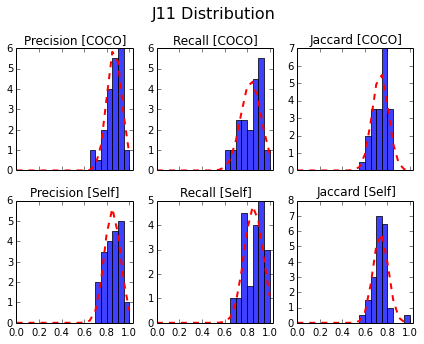
\includegraphics[width=0.45\linewidth]{plots/J11Wide.png}
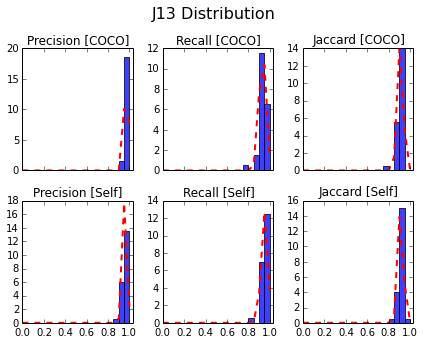
\includegraphics[width=0.45\linewidth]{plots/J13Narrow.png}
\caption{Proposed probabilistic graphical model for crowdsourcing image segmentation.}
\end{figure}
\subsubsection{Testing Assumption 3: Influence of task difficulty on spread}
\par From the Gaussian form of $\Phi$, we are interested in testing our hypothesis that if work quality exhibits a large spread, that means that the object i is probably very hard to annotate. If we exclude difficult task due to task ambiguity, we hypothesize that the number of points in the image object(as a measure of boundary complexity) should depend on the standard deviation of the fitted Gaussian. While this assumption qualitatively holds true, the Pearson's correlation coefficient and linear fits shows that there is \textbf{no linear relationship between the number of points in an object and the standard deviation of the fitted Gaussian}.

\begin{table}[h]
\centering
\begin{tabular}{lrrrrrr}
\hline
                              &   Precision[C] &   Recall[C] &   Jaccard[C] &   Precision[S] &   Recall[S] &   Jaccard[S] \\
\hline
 Average             &   0.19 &  -0.17 &   0.11 &   0.20 &   0.25 &   0.04 \\
Ground Truth &   0.03 &  -0.18 &  -0.03 &  -0.07 &   0.02 &  -0.07 \\
\hline
\end{tabular}
\caption{Pearson's linear correlation coefficient when compared to $\texttt{Average}$ (average number of points in BB drawn by all worker) and  $\texttt{Ground Truth}$ (number of points in BB drawn by me). [C],[S] short for [COCO] and [Self].}
\end{table}
\subsection{Beyond Area-based $\Phi$ functions}
\par While precision, recall, and majority-vote are simple metrics, since they are bounded by [0,1], metrics computed against BBG should always be 1. In addition these projection functions do not capture the full resolution of the bounding box.  
\subsubsection{Euclidean Distance Score}
\par \cite{Vittayakorn2011} proposes a bipartite-matching measure based on the Euclidean distance between two BBs. First, they randomly sample m=300 points along the annotation boundary, then compute all pairwise Euclidean distance. Then, the Kuhn-Munkres algorithm is used to match together the orientation of the two annotations, and returns the assignments that yields the minimum Euclidean. Finally, the score of an annotation i is computed as:
\begin{equation}
score = 1-\frac{dist_i}{max(dist)}
\end{equation},where max(dist) is the maximum Euclidean distance of all the annotations computed in our dataset. Our implementation differs slightly in that we conduct a B-spline parametric interpolation of use m=50 points along the boundary rather than random sampling, in order to speed up the computation in the Munkres algorithm. These implementation details should have little effect on the Euclidean scores computed.

\bibliographystyle{plain}
\bibliography{reference}
\end{document}